\lstdefinestyle{mystyle}{
    backgroundcolor=\color{backcolour},   
    commentstyle=\color{codegreen},
    keywordstyle=\color{magenta},
    numberstyle=\tiny\color{codegray},
    stringstyle=\color{codepurple},
    basicstyle=\ttfamily\footnotesize,
    breakatwhitespace=false,         
    breaklines=true,                 
    captionpos=b,                    
    keepspaces=true,                 
    numbers=left,                    
    numbersep=5pt,                  
    showspaces=false,                
    showstringspaces=false,
    showtabs=false,                  
    tabsize=2
}

\begin{frame}[fragile]
    \frametitle{K Nearest Neighbor Regression}

    \begin{columns}
      \column{0.5\textwidth}
      \textbf{Goal}: given $x \in \R^d$, predict sales.
      \begin{itemize}
          \item Find $k$ nearest data points to $x$.
          \item Compute the predicted sales based on these $k$ points.
      \end{itemize}
      \begin{lstlisting}[language=Python]
from sklearn.neighbors import KNeighborsRegressor
model = KNeighborsRegressor(n_neighbors=k).fit(X_train, Y_train)
res = model.predict(X_test, Y_test)
      \end{lstlisting}\pause

      \column{0.5\textwidth}
      Questions we should think about:
      \begin{itemize}
          \item How to determine $k$?
          \item How to find the nearest points efficiently?
          \item How to predict the sales based on the points?
      \end{itemize}
    \end{columns}
  
  \end{frame}

\begin{frame}[fragile]
    \frametitle{Cross Validation}
    How to determine $k$?
    \begin{itemize}
        \item Divide the training dataset into two parts $*$
        \item K-fold cross validation: divide the data into $p$ equal parts
        \begin{itemize}
            \item $\epsilon_p(k) = \sum_{i \in p\text{th part}} (y_i - f(x_i))^2$
            \item $\epsilon(k) = \frac{1}{p} \sum_{i = 1}^p \epsilon_p(k)$
        \end{itemize}
    \end{itemize}
    \begin{figure}[H]
        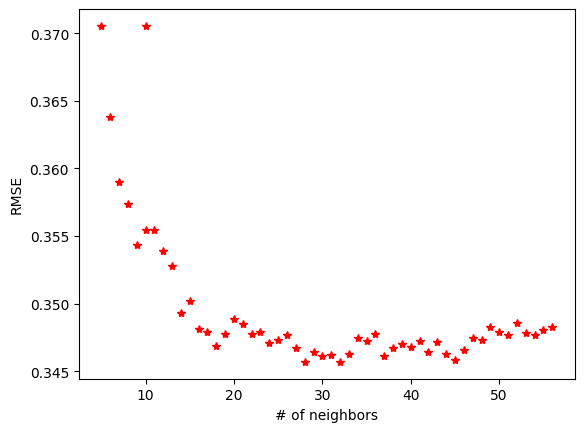
\includegraphics[scale=0.45]{graphs/knn_choice_n.png}
    \end{figure}
\end{frame}

\begin{frame}[fragile]
    \frametitle{Kd-Tree}
    How to find the nearest points efficiently given that the training size is $n$ with dimension $d$, assuming that we are using the Euclidean metric?
    \begin{columns}
    \column{0.5\textwidth}
    \begin{itemize}
        \item Naive approach
        \begin{itemize}
            \item Compare with all data points in the training set
            \item Time Complexity: $\Theta(nd)$
        \end{itemize}\pause
        \item Kd-Tree
        \begin{itemize}
            \item Construct a Kd-Tree by recursively partition the plane to two halves and balancing it.
            \item Search in a bushy binary tree
            \item The number of features we use is small.
            \item Time Complexity: $\Theta(d\log n)$.
        \end{itemize}
    \end{itemize}
    \column{0.5\textwidth}
    \begin{figure}
        \href{https://www.cs.princeton.edu/courses/archive/spring18/cos226/demos/99DemoKdTree.pdf#page=27}{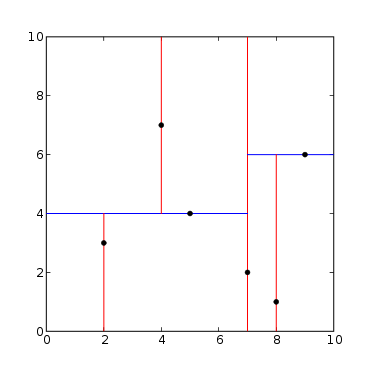
\includegraphics[scale=0.35]{graphs/kd-tree.png}}
    \end{figure}
    \end{columns}
\end{frame}

\begin{frame}[fragile]
    \frametitle{Sales Prediction}
    Given $(x_1, y_1), \ldots, (x_k, y_k)$, and $x$, how should we predict sales based on nearest points?
    \begin{itemize}
        \item \textcolor{red}{Weighted Mean}
        \begin{itemize}
            \item $d_{\text{total}} = \sum_{i = 1}^k d(x, x_i)$
            \item $y = \sum_{i = 1}^{k} \frac{d(x, x_i) y_i}{d_{\text{total}}}$
        \end{itemize}
        \item Median
        \item Linear Regression
    \end{itemize}
\end{frame}

\begin{frame}[fragile]
    \frametitle{Results}
    For our purposes, we used the K Nearest Neighbors Regressor from sklearn with Kd-Tree and weighted distance for prediction. (RMSE: 0.33)
    \begin{columns}
        \column{0.4\textwidth}
        \begin{itemize}
            \item Pros
            \begin{itemize}
                \item No assumptions about the data
            \end{itemize}
            \item Cons
            \begin{itemize}
                \item Localized data when $k$ increases ($k = 20$ in this case).
                \item Memory inefficient and slow
            \end{itemize}
        \end{itemize}
        \column{0.6\textwidth}
        \begin{figure}
            \centering
            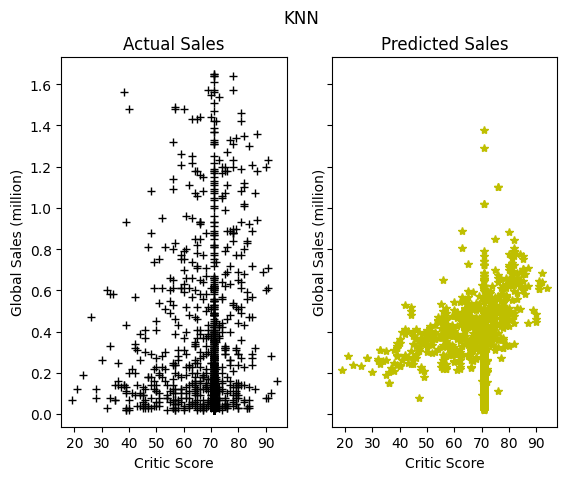
\includegraphics[scale=0.45]{graphs/knn.png}
        \end{figure}
    \end{columns}
\end{frame}